% Options for packages loaded elsewhere
\PassOptionsToPackage{unicode}{hyperref}
\PassOptionsToPackage{hyphens}{url}
%
\documentclass[
]{article}
\usepackage{amsmath,amssymb}
\usepackage{lmodern}
\usepackage{iftex}
\ifPDFTeX
  \usepackage[T1]{fontenc}
  \usepackage[utf8]{inputenc}
  \usepackage{textcomp} % provide euro and other symbols
\else % if luatex or xetex
  \usepackage{unicode-math}
  \defaultfontfeatures{Scale=MatchLowercase}
  \defaultfontfeatures[\rmfamily]{Ligatures=TeX,Scale=1}
  \setmainfont[]{SourceSansPro}
\fi
% Use upquote if available, for straight quotes in verbatim environments
\IfFileExists{upquote.sty}{\usepackage{upquote}}{}
\IfFileExists{microtype.sty}{% use microtype if available
  \usepackage[]{microtype}
  \UseMicrotypeSet[protrusion]{basicmath} % disable protrusion for tt fonts
}{}
\makeatletter
\@ifundefined{KOMAClassName}{% if non-KOMA class
  \IfFileExists{parskip.sty}{%
    \usepackage{parskip}
  }{% else
    \setlength{\parindent}{0pt}
    \setlength{\parskip}{6pt plus 2pt minus 1pt}}
}{% if KOMA class
  \KOMAoptions{parskip=half}}
\makeatother
\usepackage{xcolor}
\IfFileExists{xurl.sty}{\usepackage{xurl}}{} % add URL line breaks if available
\IfFileExists{bookmark.sty}{\usepackage{bookmark}}{\usepackage{hyperref}}
\hypersetup{
  pdftitle={Molecular Mechanisms for Human Diseases: Lab 1},
  hidelinks,
  pdfcreator={LaTeX via pandoc}}
\urlstyle{same} % disable monospaced font for URLs
\usepackage[margin=1in]{geometry}
\usepackage{graphicx}
\makeatletter
\def\maxwidth{\ifdim\Gin@nat@width>\linewidth\linewidth\else\Gin@nat@width\fi}
\def\maxheight{\ifdim\Gin@nat@height>\textheight\textheight\else\Gin@nat@height\fi}
\makeatother
% Scale images if necessary, so that they will not overflow the page
% margins by default, and it is still possible to overwrite the defaults
% using explicit options in \includegraphics[width, height, ...]{}
\setkeys{Gin}{width=\maxwidth,height=\maxheight,keepaspectratio}
% Set default figure placement to htbp
\makeatletter
\def\fps@figure{htbp}
\makeatother
\setlength{\emergencystretch}{3em} % prevent overfull lines
\providecommand{\tightlist}{%
  \setlength{\itemsep}{0pt}\setlength{\parskip}{0pt}}
\setcounter{secnumdepth}{-\maxdimen} % remove section numbering
\usepackage[default]{sourcesanspro}
\usepackage[T1]{fontenc}
\ifLuaTeX
  \usepackage{selnolig}  % disable illegal ligatures
\fi

\title{Molecular Mechanisms for Human Diseases: Lab 1}
\usepackage{etoolbox}
\makeatletter
\providecommand{\subtitle}[1]{% add subtitle to \maketitle
  \apptocmd{\@title}{\par {\large #1 \par}}{}{}
}
\makeatother
\subtitle{Bacteria's Brain -- Part A}
\author{}
\date{\vspace{-2.5em}}

\begin{document}
\maketitle

{
\setcounter{tocdepth}{2}
\tableofcontents
}
Analysis:

\begin{verbatim}
## # A tibble: 18 x 2
##        t concentration
##    <dbl>         <dbl>
##  1 0.170        0.019 
##  2 0.443        0.0855
##  3 0.511        0.116 
##  4 0.716        0.164 
##  5 1.06         0.247 
##  6 1.20         0.280 
##  7 1.43         0.328 
##  8 1.65         0.356 
##  9 1.83         0.404 
## 10 2.11         0.454 
## 11 2.42         0.506 
## 12 3.00         0.615 
## 13 3.68         0.675 
## 14 4.23         0.713 
## 15 4.83         0.798 
## 16 5.41         0.760 
## 17 6.06         0.860 
## 18 6.66         0.874
\end{verbatim}

\begin{verbatim}
## # A tibble: 20 x 2
##        t concentration
##    <dbl>         <dbl>
##  1  2.38       0.0109 
##  2  2.72       0.00934
##  3  3.04       0.0146 
##  4  3.52       0.0145 
##  5  4.00       0.0242 
##  6  4.57       0.0286 
##  7  5.05       0.0376 
##  8  5.54       0.0435 
##  9  6.45       0.0592 
## 10  7.53       0.0764 
## 11  8.58       0.107  
## 12  9.63       0.118  
## 13 10.8        0.128  
## 14 12.0        0.16   
## 15 13.2        0.188  
## 16 14.3        0.199  
## 17 22.7        0.317  
## 18 24.9        0.349  
## 19 26.8        0.378  
## 20 28.9        0.408
\end{verbatim}

Visualization of Data set A

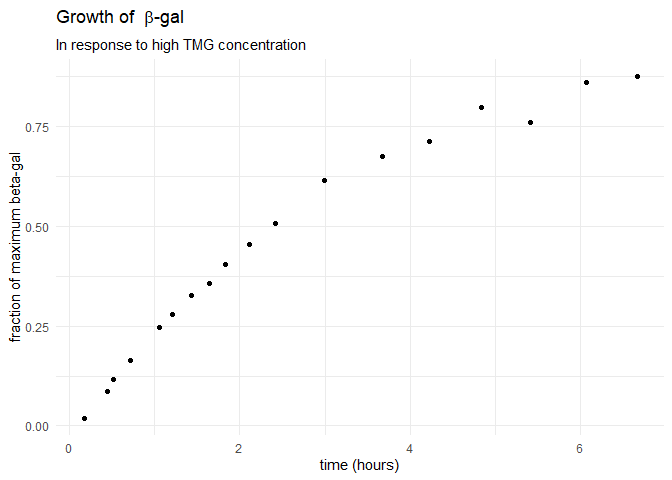
\includegraphics{bacterias_brain_files/figure-latex/a_Q1-1.pdf}

Fitting function on Data set A

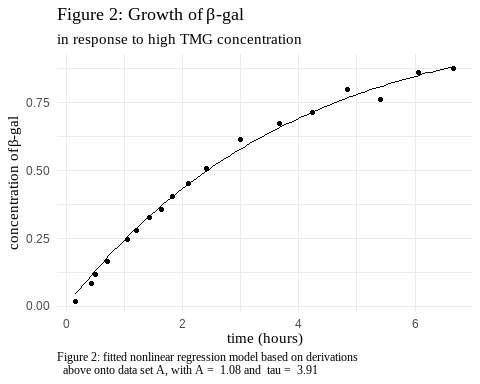
\includegraphics{bacterias_brain_files/figure-latex/a_q2-1.pdf}

\begin{verbatim}
##            ampl      tau
## .       1.07972 3.907721
## coef_a3 1.07972 3.907721
\end{verbatim}

\begin{verbatim}
## 
## Formula: a_q3_df$concentration ~ growth_a(t, ampl, tau)
## 
## Parameters:
##      Estimate Std. Error t value Pr(>|t|)    
## ampl  1.07972    0.03931   27.47 1.59e-15 ***
## tau   3.90772    0.24889   15.70 1.50e-11 ***
## ---
## Signif. codes:  0 '***' 0.001 '**' 0.01 '*' 0.05 '.' 0.1 ' ' 1
## 
## Residual standard error: 0.02143 on 17 degrees of freedom
## 
## Number of iterations to convergence: 5 
## Achieved convergence tolerance: 1.242e-06
\end{verbatim}

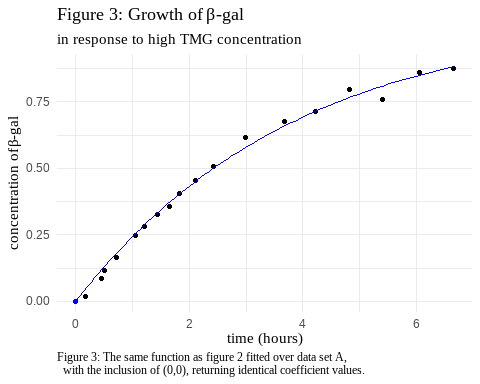
\includegraphics{bacterias_brain_files/figure-latex/a_q3-1.pdf}

Analysis:

Visualization of Data set B

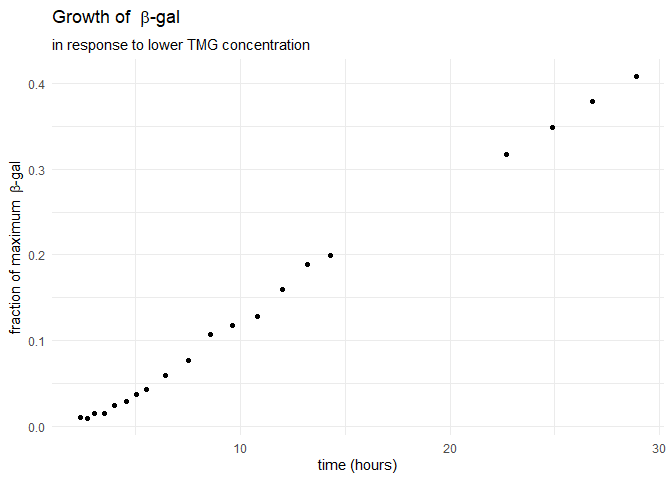
\includegraphics{bacterias_brain_files/figure-latex/b_q1-1.pdf}

Fitting function on Data set B

\begin{verbatim}
## (Intercept)      b_q2$t 
## -0.09474840  0.02094596
\end{verbatim}

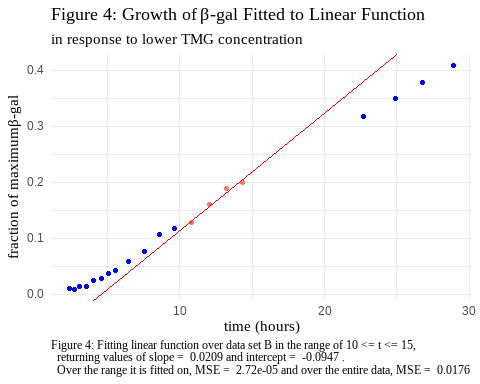
\includegraphics{bacterias_brain_files/figure-latex/b_q2-1.pdf}

\begin{verbatim}
## 
## Call:
## lm(formula = b_q2$concentration ~ b_q2$t)
## 
## Residuals:
##         1         2         3         4 
## -0.004175  0.002961  0.007005 -0.005791 
## 
## Coefficients:
##              Estimate Std. Error t value Pr(>|t|)  
## (Intercept) -0.094748   0.036016  -2.631    0.119  
## b_q2$t       0.020946   0.002847   7.356    0.018 *
## ---
## Signif. codes:  0 '***' 0.001 '**' 0.01 '*' 0.05 '.' 0.1 ' ' 1
## 
## Residual standard error: 0.007376 on 2 degrees of freedom
## Multiple R-squared:  0.9644, Adjusted R-squared:  0.9465 
## F-statistic: 54.11 on 1 and 2 DF,  p-value: 0.01798
\end{verbatim}

\begin{verbatim}
## Warning: 'newdata' had 20 rows but variables found have 4 rows
\end{verbatim}

\begin{verbatim}
## # A tibble: 2 x 2
##         MSE data          
##       <dbl> <chr>         
## 1 0.0000272 10<= t <= 15  
## 2 0.0176    entire dataset
\end{verbatim}

As we can see, the Mean Standard Error (MSE) for the model fits well
within the range of 10\textless= t \textless= 15, but not well over the
entire data set.

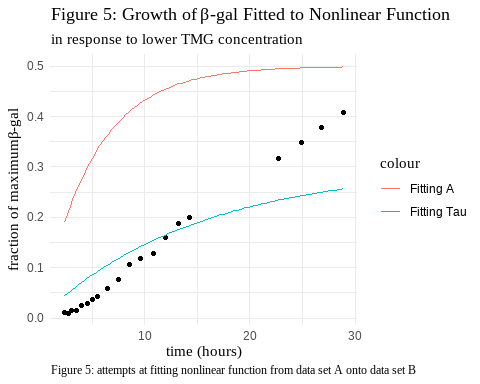
\includegraphics{bacterias_brain_files/figure-latex/b_q3-1.pdf}

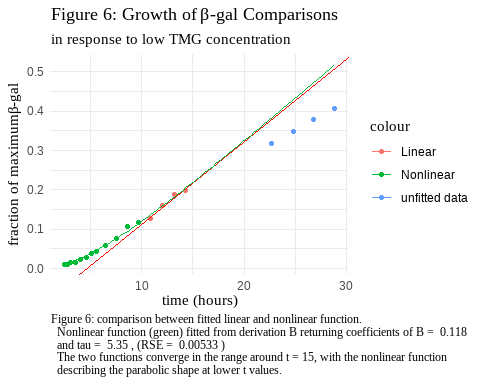
\includegraphics{bacterias_brain_files/figure-latex/b_q4-1.pdf}

Q5: at large t, the function becomes linear as -t/tau becomes 0 so
exp(-t/tau) becomes a constant of 1

Analysis:

\end{document}
